\documentclass{sig-alternate-10pt}
%\documentclass[letterpaper,11pt]{article}
\usepackage{url}
%\usepackage{usenix,epsfig,endnotes}
%\usepackage{fullpage} 
%\setlength{\textheight}{9in}
%\setlength{\textwidth}{6.75in}
%\setlength{\oddsidemargin}{-.125in}
\usepackage{graphicx}
%\usepackage{subfigure}
%\usepackage{ifpdf}
%\usepackage{multicol}
%\usepackage{amsmath, amssymb, amsthm}
%\usepackage{rotating}
\usepackage{multirow}
\usepackage{rotating}
%\onehalfspacing

%COMMENT FOR FINAL VERSION
%\newcommand{\tbd}[1]{[{\bf{#1}}]}
%\newcommand{\justine}[1]{[{\bf justine: {#1}}]}
%\newcommand{\shaddi}[1]{[{\bf shaddi: {#1}}]}
%\newcommand{\kristin}[1]{[{\bf kristin: {#1}}]}

%UNCOMMENT FOR FINAL VERSION
\newcommand{\tbd}[1]{}
\newcommand{\justine}[1]{}
\newcommand{\shaddi}[1]{}
\newcommand{\kristin}[1]{}


\newcommand{\ie}{{\it i.e.}}
\newcommand{\eg}{{\it e.g.}}
\newcommand{\eat}[1]{}

%\newcommand{\tbd}[1]{}
%\setlength\topmargin{0in}
%\usepackage{verbatim}
%\usepackage[compact]{titlesec}
%\usepackage[small]{caption}
\usepackage{times}
%\titlespacing{\section}{0pt}{*0}{*0}
%\titlespacing{\subsection}{0pt}{*0}{*0}
%\titlespacing{\subsubsection}{0pt}{*0}{*0}
%\titlespacing{\abstract}{0pt}{*0}{*0}
%%REPLACES ITEMIZE

\title{Modeling Regional Failures in Interdomain Connectivity}
\author{\begin{tabular}{ccc} Shaddi Hasan & Justine Sherry & Kristin Stephens\\
%        \begin{multicols}{2}{{\it Draft - Please do not distribute.}}\\
        \end{tabular}\\
    University of California, Berkeley\titlenote{Authors listed
    alphabetically.}\\\\
        \large
        {\it CS270 Final Project}}
        \normalsize
%\author{Paper \#69, 14 Pages}
\date{}
\begin{document}    
    \maketitle

        %Internet interdomain resilience requires engineering for failure, from
        %deploying robust routing protocols, to establishing logical
        %connectivity redundancy (multihoming), to building redundant
        %interomain physical links.  
    \abstract{\it
        Earthquakes, hurricanes, and other regional disasters can 
        stress Internet interdomain connectivity.  Because of their widespread
        impact, these disasters can cause failures of entire exchange points or
        severance of long distance cables, leading to correlated failures in
        interdomain connectivity.  In this paper we develop a model, geodesic
        failure regionalization, to explore the impact of regional failures on
        Autonomous System (AS) connectivity.  We map logical AS connectivity links to geographic
        regions where peering occurs to model the regional redundancy of
        peering connections.
        By modeling the redundancy of logical AS
        connectivity, we can perform
        finer-grained analysis of the impact of catastrophe than work which
        relies only on logical AS connectivity alone.  
        Our data demonstrates that most transit-providing networks peer in redundant locations, such that small physical disasters ar unlikely to partition two peering networks.    
    However, our data also includes geographic regions served by only a limited number of ASes with limited peering to external networks, leaving these geographic regions suceptible to disconnection after damage to only a few regions containing all of their egress connectivity.
    }
    
    \section{Introduction}
        The United States government defines {\it critical infrastructure} as ``systems
and assets, whether physical or virtual, so vital to the United States that the
incapacity or destruction of such systems and assets would have a debilitation
impact on security, national economic security, national public health or
safety, or any combination of those matters''~\cite{patriotact}. Internet
connectivity, a fundamental requirement for modern communication, is
undoubtedly such a system.  Businesses~\cite{something?} and
governments~\cite{cyberspacepolicy} hence value the physical security of
Internet infrastructure to disaster or attack.


In this paper, we provide a brief glance at physical Internet resilience by
focusing on a model of geographic locations where multiple networks converge to
interconnect. Damage to an Internet Exchange Point (IXP) or Point-of-Presence
(PoP) are worst-case scenarios for physical disaster, as these locations
provide connectivity between anywhere from two to hundreds of networks.
Building on prior work which develops techniques for identifying formal
IXPs~\cite{ixps-mapped}, discovering PoPs in general~\cite{iplane}, and
pinpointing border routers~\cite{asbrsomething}, we develop an AS connectivity
graph that focuses on the locations where peering takes place.  We then
consider the behavior of an adversary who seeks to maximize damage to this
connectivity graph.  Such an adversary might wish to disconnect two Tier 1
networks, isolate a large number of networks, or partition a geographic region
from the rest of the Internet.  We consider each in turn.


We are not the first to evaluate Internet resilience to
failures~\cite{michigan, measuringresilience, resilience-under-BGP,
resilience-complex-networks}.  Our contribution is to consider physical
locations of conncetivity as {\it failure points}.  Previous work focused on
the impact of severing logical links, that is, declaring that two networks had
been entirely disconnected.  This overestimates realistic damage in some cases,
and underestimates in others.  For example, it is highly unlikely that two Tier
1 networks would be partitioned in any single event.  These networks have
global footprints and connect at multiple physical locations.  Thus,
disconnecting Tier 1 networks is an overestimate of damage in all scenarios
except a coordinated attack.  On the other hand, disconnecting logical links
one by one ignores the physical reality that any disaster that strikes a link
in shared infrastructure such as an IXP is likely to impact a large number of
links.  In this case, modeling failure of a single logical link is an
underestimate.  We argue that focusing on physical connectivity points is a
more realistic model of the impact of physical disaster. 

\eat{ Not true!
 
Second, we consider resilience in an adversarial setting.  Recent events in
Egypt~\cite{thenews} and other countries involved government intervention to
sever Internet access in order to limit communication between revolutionaries
and the outside world.  Further, the criticality of Internet communication
makes it a prime target for terrorist attack.  Attacks by any human entity may
involve damage to one or more physical locations.  Hence, our analysis is a
superset of previous work which focused primarily on natural disaster or
sideffects from events in a single location.
}

Before we move forward, we clarify the scope of our goals.  
Evaluations of AS-level connectivity graphs show that traceroute-based
topologies like those that we rely upon are in many ways
incomplete~\cite{walter}.  For instance, policy compliant routing ensures that
measurements made with only limited vantage points cannot observe peering
relationships between networks where neither network contains a measurement
vantage point.  Further, `backup links', which are provisioned for the case of
failure but otherwise unused, cannot be observed since no traffic flows across
these links when the primary links are available.  These and other impediments
mean that any analysis over measurement-based graphs may be missing critical
information.  Thus, the results of our study should not be considered hard and
fast projections of Internet connectivity.  Instead, we aim only to provide
{\it estimates} and {\it bounds} on the impact of attack on Internet
infrastructure.

Our results estimate that \ldots \justine{My hypotheses: (1) we find that
Tier-1's are too well connected to feasibly partition - we can echo the
argument from that paper Kristin found that the threat is misconfiguration or
attacks on the control plane, but certainly not the physical infrastructure.
(2) The exact opposite is true for small networks - that taking out a single
IXP in many cases is enough to knock offline dozens of ASes and hundreds or
thousands of prefixes. WRT geographic regions, I am less sure - hopefully we
can identify the Egypts of the world?}

The remainder of the paper is organized as follows.
Section~\ref{sec:connectivity} discusses our dataset and model of the physical
connectivity of Internet infrastructure.  Section~\ref{sec:algos} provides the
algorithms we used in analyzing this model.  Section~\ref{sec:results}
describes our discoveries from applying these algorithms.  Finally, we discuss
related work in \S~\ref{sec:relatedwork} and conclude in
\S~\ref{sec:conclusion}.



    \section{Connectivity Model}
        \label{sec:connectivity_model}
            In order to study the impact of regional disaster, we augment a standard AS logical connectivity graph~\cite{caida-asgraph} with measurements of the geographic regions in which networks peer.
    We model the Earth as a geodesic globe inscribed in a sphere of the Earth's radius, and map latitude and longitude values to a face on the globe.
    We consider each face of the globe as a `region,' such that a worst-case disaster could destroy all of the physical routing infrastructure within the region.
    We generate the geodesic globe using a standard algorithm~\cite{geodesic}, providing us with \shaddi{?} \shaddi{triangular?} cells, each with average width of \shaddi{?}km and area \shaddi{?} km$^2$.  
    Dividing the globe in to cells allows us to cleanly model the concept of a `region' - a region is one cell, or a set of contiguous cells, all suceptible to the impact of shared event. 
     
    We map every location where peering takes place to a cell on the globe, and use the resulting grid to perform our analysis of interdomain connectivity.
    We generate peering locations using a combination of an Internet Exchange Point dataset~\cite{ixps-mapped}, and observed router-level AS adjacencies from the CAIDA Internet Topology Data Kit (ITDK)~\cite{itdk}.
    The ITDK is a router-level Internet map generated from traceroute, mrinfo, and other active measurement data.
    The dataset provides geolocations for each router provided by the MaxMind~\cite{maxmind} commercial geolocation database.
    Because small ASes typically have only one or two providers and are limited in their geographic extent, we remove `stub' ASes from our dataset entirely, limiting our analysis to networks who provide transit to other networks.
    Because commercial geolocation techniques are on average incorrect by 100 km~\cite{someone}, our mapping to \shaddi{n} km wide cells ensures that the average geolocated peering is either in its proper cell, or a cell adjacent to its proper cell.
    
    
    Figure~\ref{fig:worldmap} illustrates our model and our data.
    We observe that cell density is heavier in the United States and Europe, which is consistent with the higher density of Internet connectivity in these regions compared to the rest of the world.
    However, this also may be an artifact of the limitations of commercial geolocation, which provide better city-level granularity in Europe and the United States than in other areas of the world, where IP addresses are more likely to map to the capitol city of their country.
    We also observe...\shaddi{?} 

\eat{ 
    We develop our peering dataset by borrowing techniques and data from
    the IXP
    Mapping Project~\cite{ixps-mapped}, iPlane~\cite{iplane},
    Aqualab~\cite{sidewalk},
    CAIDA~\cite{caidadata}, and the MaxMind~\cite{maxmind} industrial IP geolocation service.
    For the iPlane and Aqualab data, we derive peering points from raw traceroute files.
    For each pair of IP addresses we observe adjacent in a traceroute, we map the IPs to alias clusters generated by CAIDA's iffinder~\cite{iffinder} and MIDAR~\cite{iffinder, midar} measurements.
    We then map the alias clusters to ASes, and if the ASes are different, we store the two IP addresses as an AS peering.
    Since the majority of stub networks are not geographically widespread, we limited our study to networks which provided transit to at least one AS; thus, we removed any adjacency which included a stub network.
    We map the peering to a geographic location using a combination of DNS-based geolocation and the MaxMind commercial geolocation service.
    For both IP addresses in the adjacency, we do reverse DNS lookups on all IP addresses in their alias clusters. 
    If any of the DNS names match rules from the undns~\cite{undns} or sarang~\cite{sarang} projects, we map the IP address to that location. 
    If multiple of the IP addresses point to different locations, we elect the most common location, or in a tie, choose the location with the least distance from the others.
    If no DNS names are found, we repeat the same process with locations from the MaxMind GeoLite City database, which has better coverage that DNS geolocation, but worse accuracy~\cite{uhlig_ccr_paper}. 
    
    The measurements we gathered from CAIDA, iPlane, and Aqualab allowed us to identify 489,334 router-level AS adjacencies, which we mapped to 14,457 unique latitude, longitude locations (133,686 using DNS, and the remainder using MaxMind).
    We then supplemented these measured adjacencies with 38,994 adjacencies from a ground-truth dataset~\cite{ixps-mapped}, bringing our total to 528,328 adjacencies in 14,571 uniqe latitude, longitude locations. 
    We mapped these adjacencies to 2,900 unique faces of the geodesic globe.   

 
        \subsubsection*{Evaluation of Model}

            To evaluate the representativeness of our data, we investigate the fraction of logically connected ASes for whch we were able to identify geolocated adjecencies, compare our measured adjacencies to a set of ground truth adjacencies, and perform a survey of network operators to validate our data.

            {\bf Representation of Logical Connectivity.} 
            Finite vantage points, policy-based routing, backup links, and limited geolocation capabilities limit our ability to exaustively discover AS adjacencies. 
            Policy-based routing means that traceroutes issued from within a network, or from a network's customer AS, may be able to traverse paths that an issuer from outside the network may not be able to traverse.
            With only finite vantage points limited to a fraction of networks, our measurements may fail to identify many AS-level links.
            Further, backup links between ASes may never be traversed by our traceroute measurements, since backup links are by definition offline unless a failure occurs on a primary link.
            Finally, since geolocation (especially for routers rather than end hosts) is limited, even when we identify an AS-level adjacency we may not be able to geolocate it.
            
            As a first step towards identifying how representative our dataset is, we count how many AS peerings our geolocated adjacencies capture vs those from more exhaustive datasets (note that ground truth data is unavailable).
            \justine{TODO: this.}

            {\bf Ground Truth Adjacencies.}
           We next take a set of `ground-truth' adjacencies, peerings with known locations, and compare them to our measured adjacencies. 
           The ground truth adjacencies are borrowed from the IXP Mapping Project~\cite{ixps-mapped}, which manually investigated every public Internet Exchange Point worldwide.
            For each adjacency, we mapped it to the measured adjacency nearest to it on the globe.
            Figure~\cite{fig:closestadjacency} shows the results in CDF form.
            We provide results for comparison to measured adjacencies geolocated using our combined techinique (DNS and Maxmind geolocations both used), DNS geolocation only, MaxMind geolocation only, and strawman geolocation in which all adjacencies are mapped to Greenwich, England.
            \justine{TODO: describe} 




            {\bf Operator Survey.} {\it Due to our poor performance on the previous two metrics, we decided to hold off on our operator survey until we have data we feel confident in sending out for operator validation.}
}




    \section{Measuring Connectivity}
        \label{sec:quant_connect}
        \eat{
\begin{figure*}
    \centering
    \begin{tabular}{ccc}
        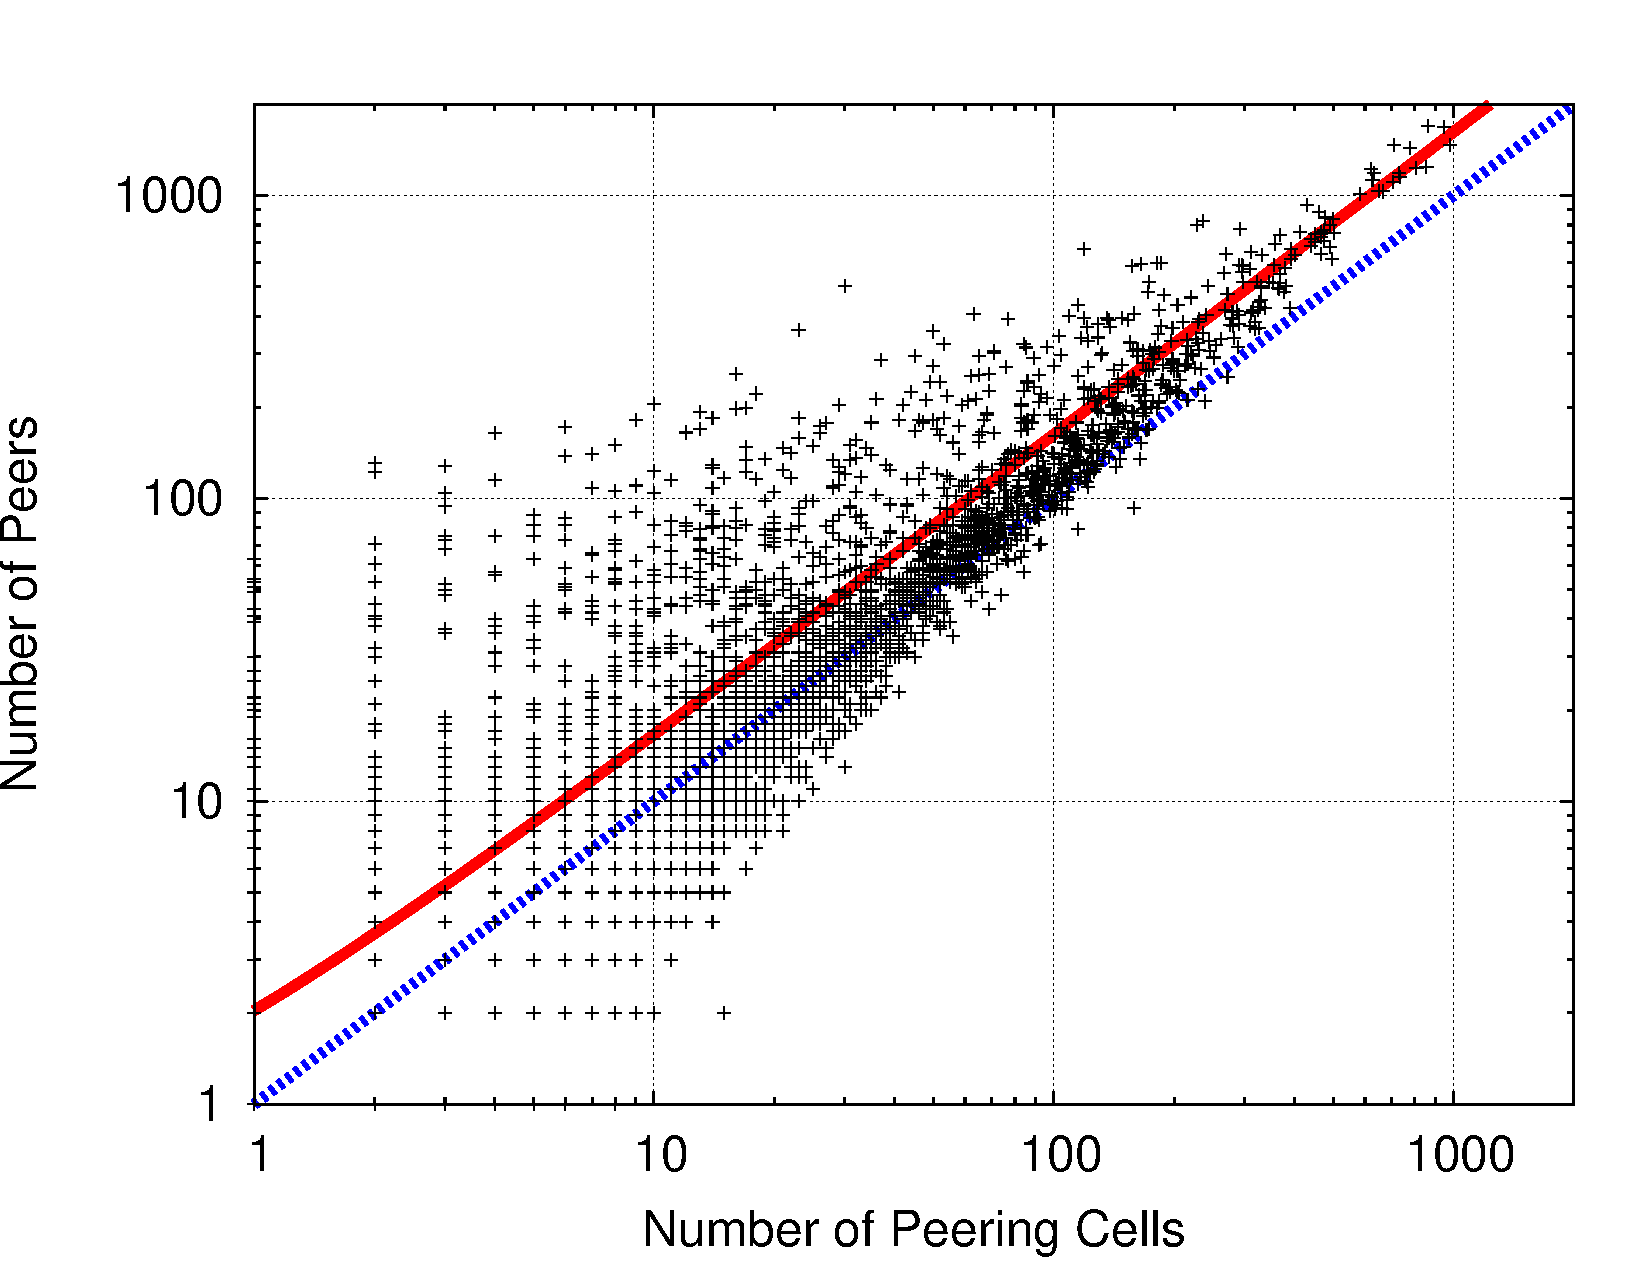
\includegraphics[width=2.2in]{scatter}&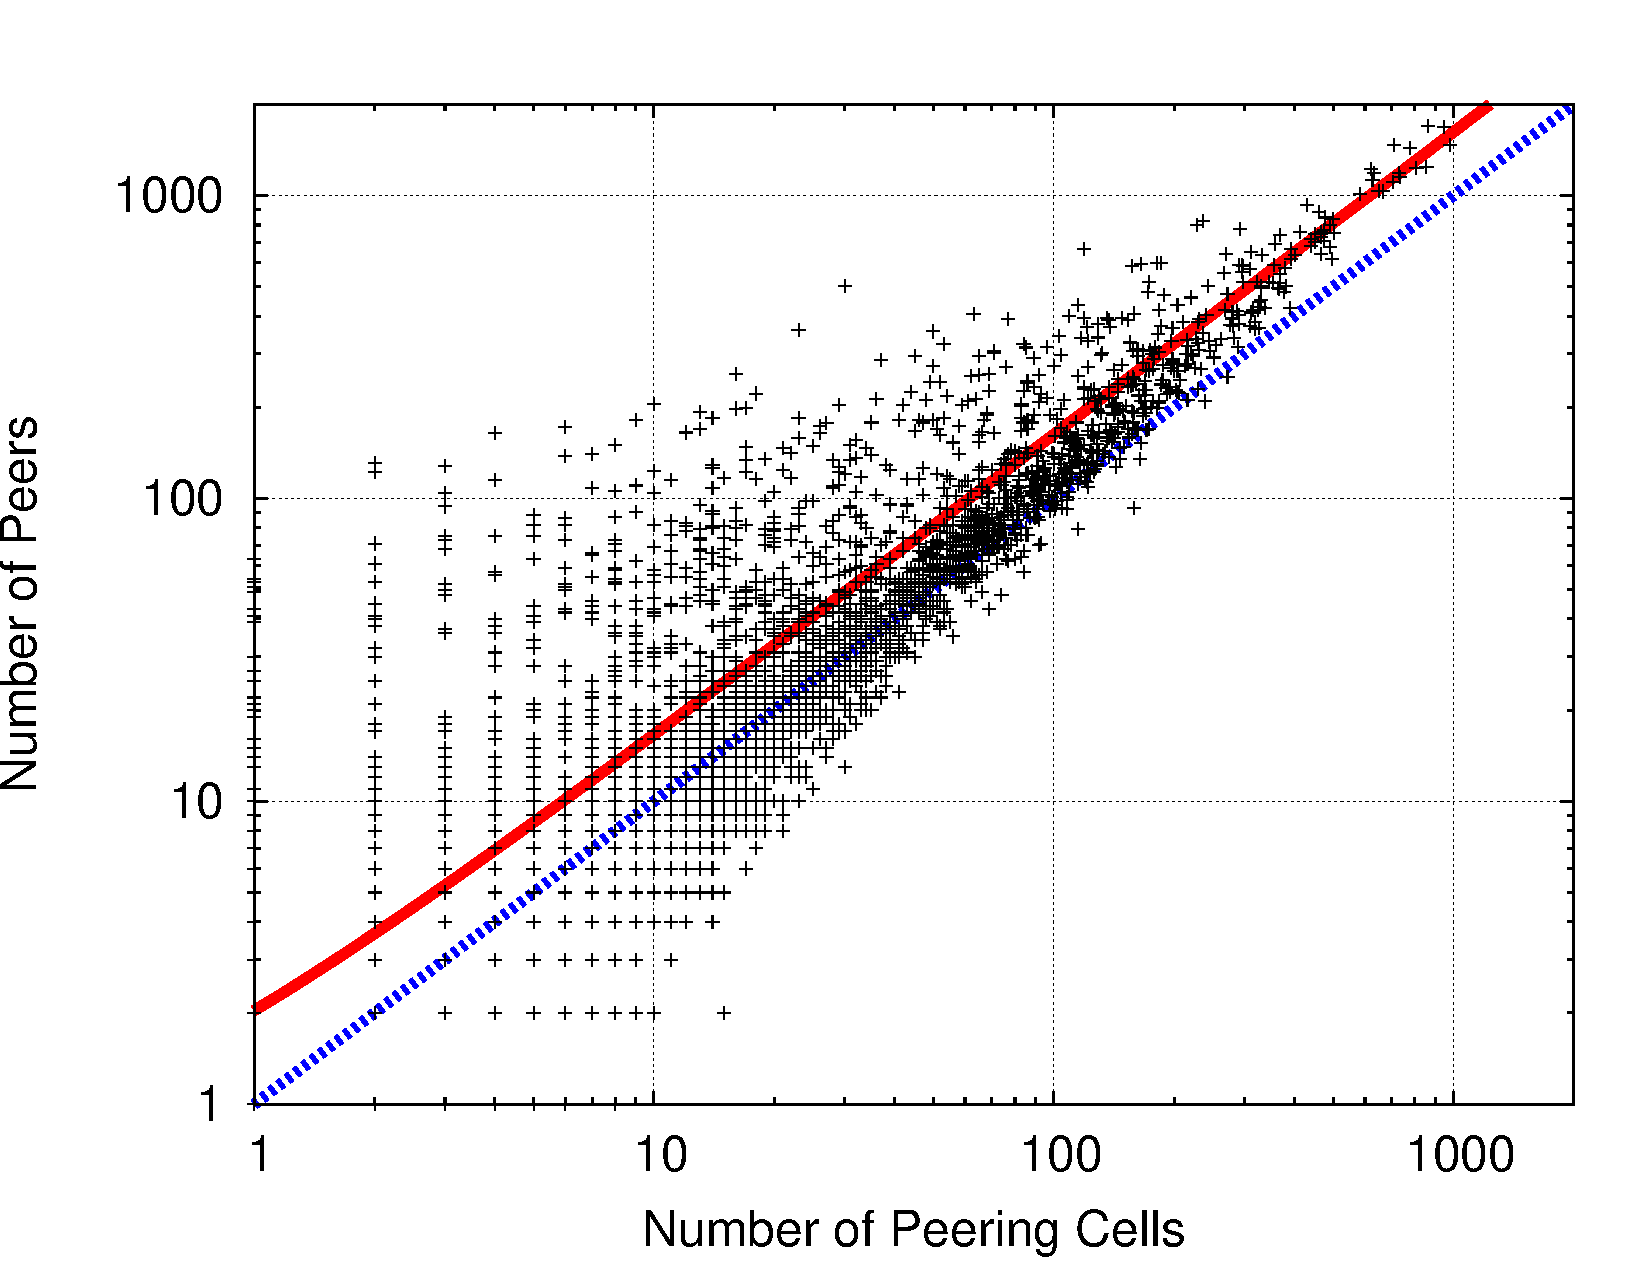
\includegraphics[width=2.2in]{scatter}&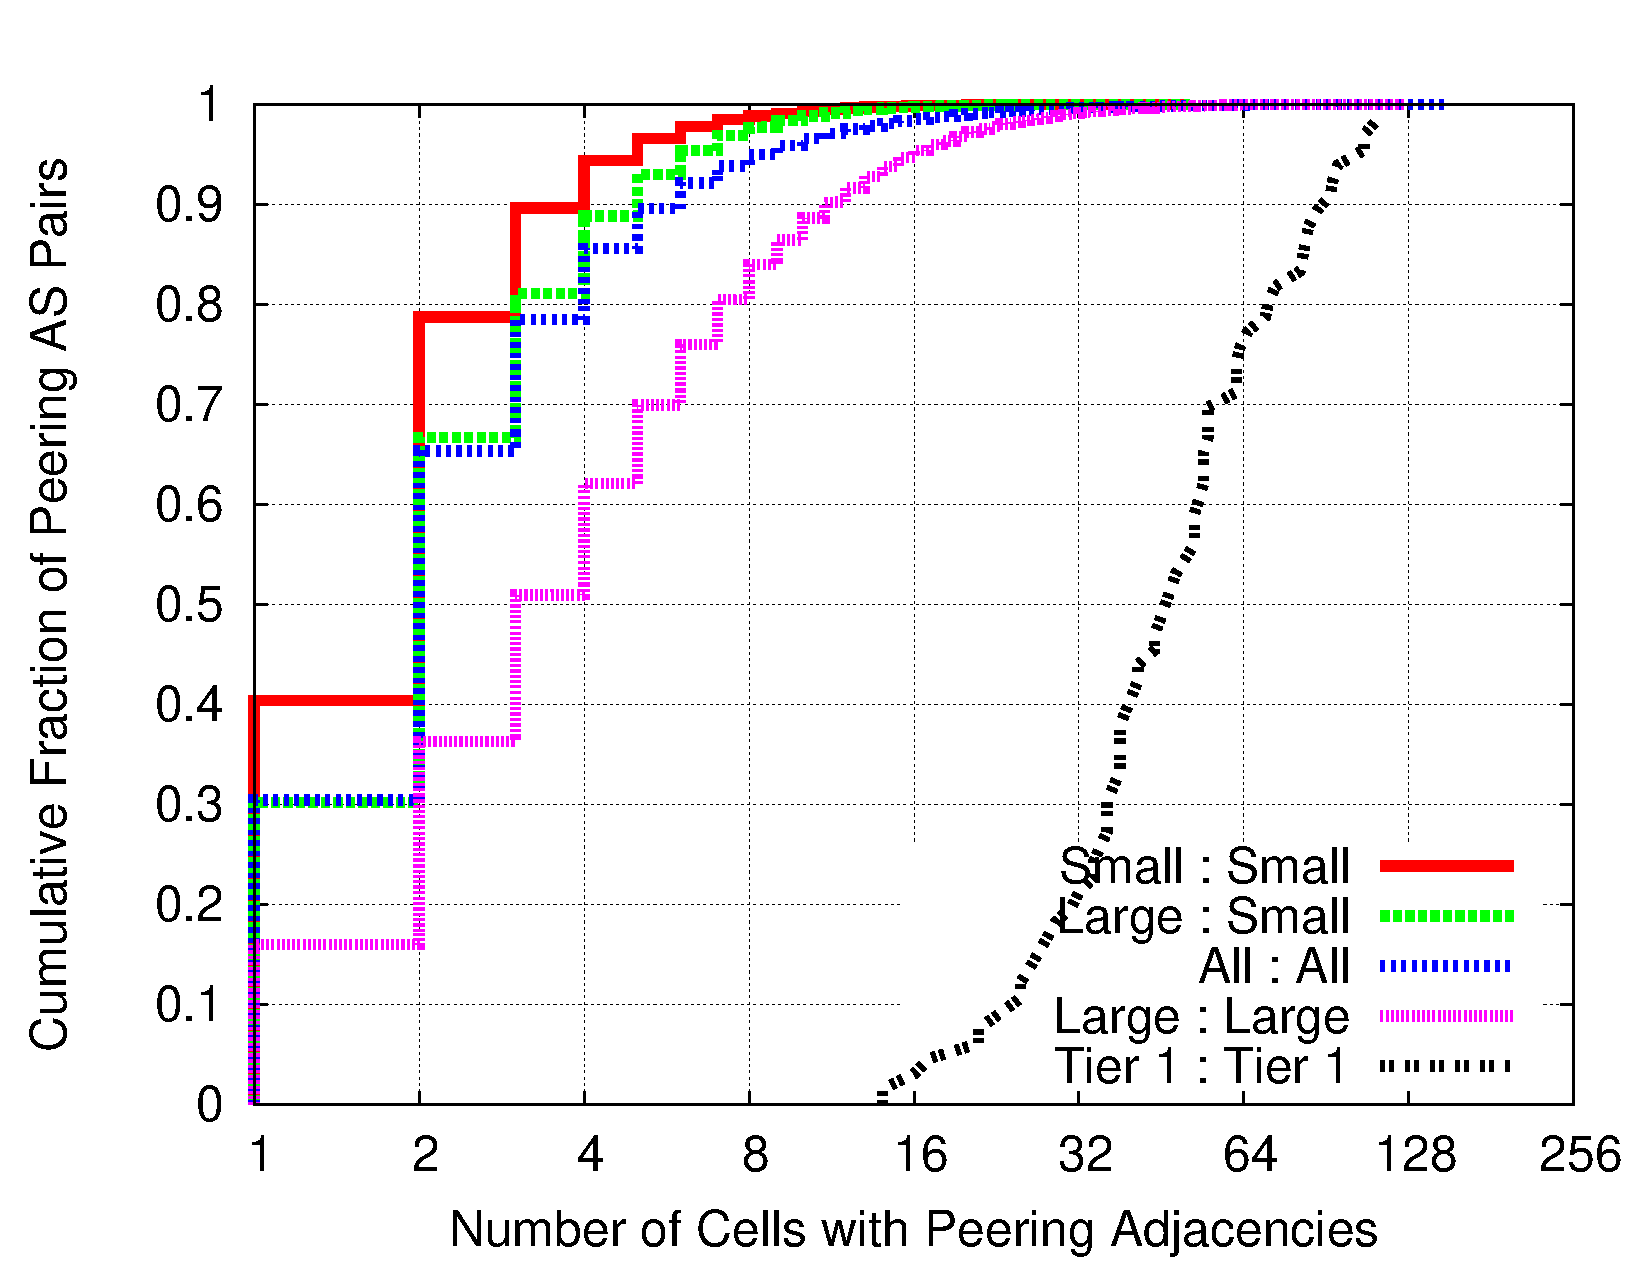
\includegraphics[width=2.2in]{peering}\\
    \end{tabular}
\end{figure*}    
}

    \begin{figure}[tb]
\centering
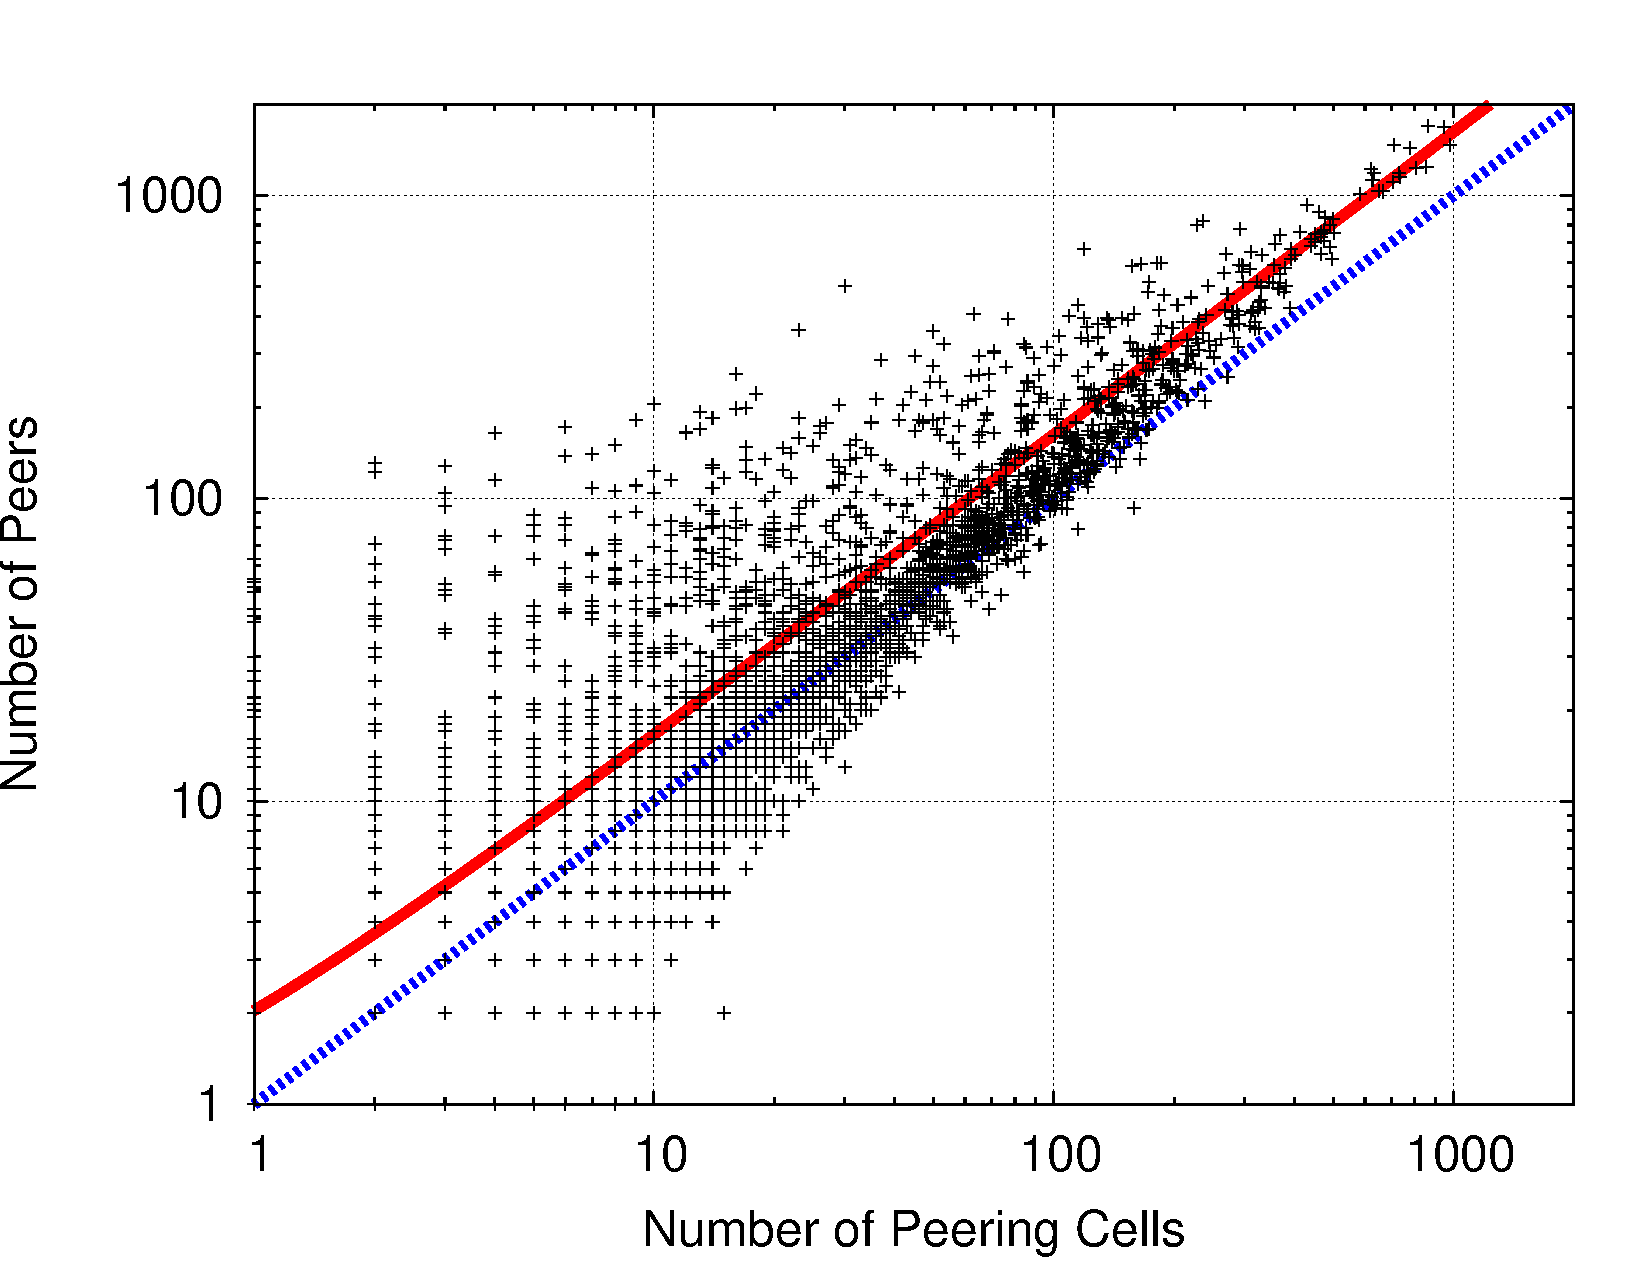
\includegraphics[width=3.25in]{scatter}
\caption[]{\label{fig:scatter} Scatter plot of observed peers to cells with peering adjacencies. Each point represents an AS which has peering in $x$ cells of the globe, with $y$ total peers. A linear regression (shown, upperline) predicts the ratio of cells to peers to be .625 in the average case. The lower line shows a 1:1 ratio.} 
\end{figure}

\begin{figure}[tb]
\centering
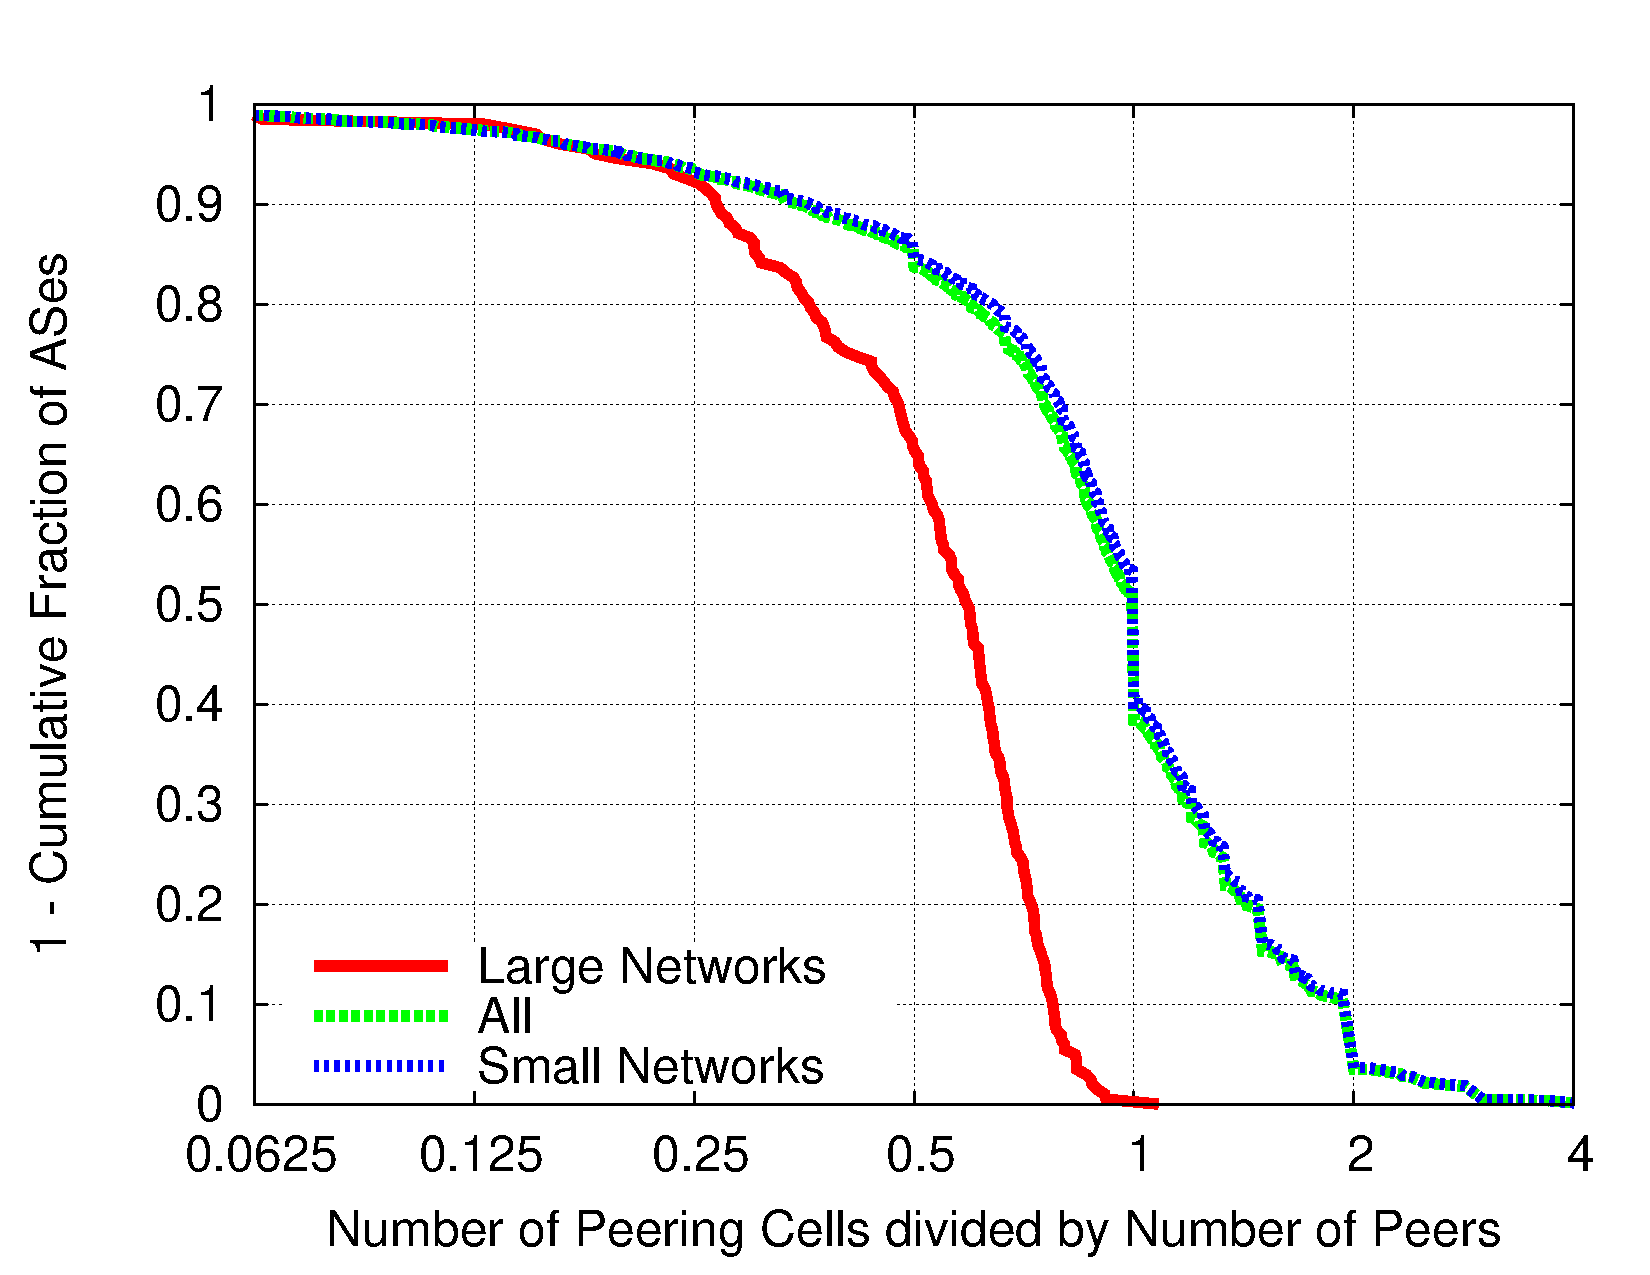
\includegraphics[width=3.25in]{ratio}
\caption[]{\label{fig:ratio} Cumulative distribution of geographic redundancy ratio: the number of cells a network peers in divided by the number of peers it has.} 
\end{figure}




 


    We now provide some basic observations about our data: the number of regions ASes peer in, and how many redundant peering locations ASes maintain per peering relationship.
    We note that, while 84\% of networks are `stub' networks that provide transit to no one, usually with few providers and limited geographic extent, we focus our analysis on networks which provide transit to other networks.
    While the failure of stub networks has no impact on the connectivity graph besides its own disconnectivity, transit networks have entire networks as customers and thus their resilience is important not only for their own connectivity, but that of other networks.

\subsubsection*{Geographic Diversity}
    We first investigate the geographic diversity of peering locations for a single AS, with attention to how the number of peering locations scales with number of neighbors a network has.
    Figure~\ref{fig:scatter} illustrates the range of values for both number of peers ($y$-axis) and number of cells in which the network connects to its peers ($x$-axis).
    We see the number of observed peers range from one (\ie{} the network's provider, since we removed stub ASes from the dataset) to well over 1000 for what must be Tier-1 networks.
    The number of peering locations ranges from one - even for networks with some tens of peers - to hundreds.
    The number of peering locations scales linearly with the number of peers; a linear regression (shown) plots the ratio  at 3 peers to one peering point. 
    However, there are a large number of ASes and the scatterplot is wide around the linear plot for smaller numbers of peers and locations.


    To better investigate this ratio, Figure~\ref{fig:ratio} shows a CCDF of the number of peering cells to number of peers for Tier 1 networks, Large networks (more than 250 peers), Small networks (less than 250 peers), and All networks. 
    Thus, a given $(x,y)$ coordinate means that $y$ fraction of of networks had a ratio larger than $x$ peers for every peering point.
    Here we observe that the average large network has a ratio of .653, while the average small network has a ratio of 1.
    This is because large networks often peer with multiple small networks with whom they only peer in a small fraction of their peering points, while smaller networks often peer with more widespread providers and in a more limited number of locations.
    \justine{This is pure bullshit. I am not sure why and we should - LATER - take time to investigate these graphs.}

\subsubsection*{Peering Redundancy}
    Networks not only maintain multiple peering relationships in multiple locations, but have redundant peering connections in different regions with the same peers.
    In Figure~\ref{fig:peering_redundancy} we plot a CDF of the number of peering cells for AS peering relationships, separating peering relationships between Tier-1 networks, Large (more than 250 peers) networks, and Small networks (less than 250 peers).
    For this graph, an $(x,y)$ point means that $y$ fraction of peering AS pairs connect to each other in less than or equal to $x$ cells on the geodesic globe.

    Since each Tier-1 network forms a large portion of the global backbone, it is no surprise that one pair peers in almost a hundred places, and the least well-connected pair of Tier-1 networks peers in some 14 places.
    Even small (less than 250 peers) networks are typically redundantly connected. 
    While 40\% of peering pairs where both networks are small networks occur in only one cell, the average pair peers in two cells and 20\% peer in three or more cells. 

    Because most transit-providing networks peer with other transit providing networks redundantly, this greatly diminishes the likelihood of a regional disaster or outage disconnecting two transit-providing networks.
    While such a disaster may have impact on intradomain connectivity, interdomain connections are at least once redundant for small transit networks, and tens of times over in the case of the largest networks.

\begin{figure}[tb]
\centering
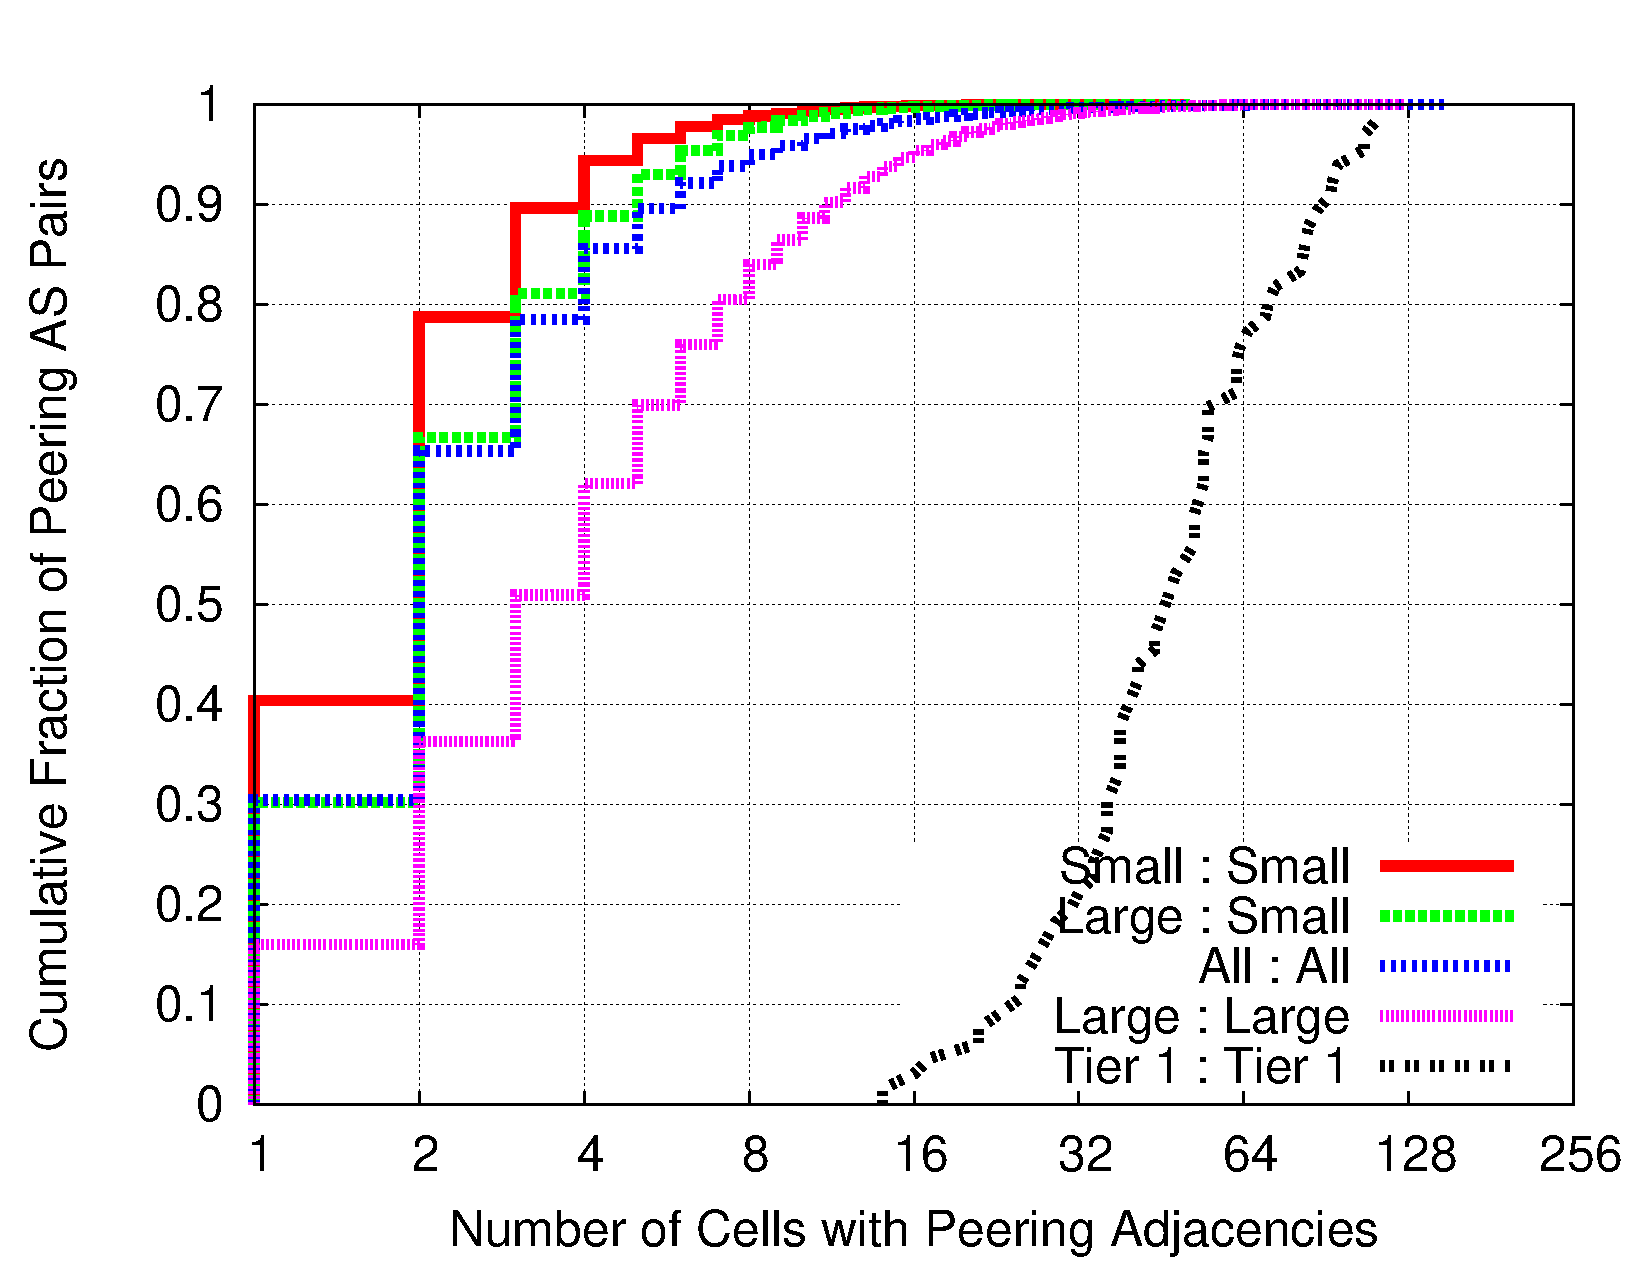
\includegraphics[width=3.25in]{peering}
\caption[]{\label{fig:peering_redundancy} Cumulative Distribution of AS Pairs with redundant regional connectivity. Only 16\% of peerings between large networks occur in only one cell, and 40\% of peerings between small networks occur in only one cell.} 
\end{figure}



    \section{Regional Failure Analysis}
        \label{sec:failures} 
            \begin{table}
        \centering
        \begin{tabular}{lc|l|l|l|l|l|l}
            &&\multicolumn{5}{c}{\bf Number of Partitions}\\
            &&{\bf 2}&{\bf 4}&{\bf 8}&{\bf 16}&{\bf 32}\\
            \hline
            \multirow{5}{*}{\begin{sideways}{\bf Imbalance (\%)}\end{sideways}}
            &{\bf 5}&1036&1520&1818&1993&2087\\
            &{\bf 10}&1045&1495&1809&1987&2085\\
            &{\bf 15}&1031&1481&1798&1981&2097\\
            &{\bf 20}&1000&1482&1787&1971&2090\\
            &{\bf 25}&986&1464&1777&1965&2085\\
        \end{tabular}
        \caption[]{\label{tbl:hmetis} Number of cells to remove in order to fully partition the network, such that no users from one partition can communicate with any user in another partition. Columns indicate the number of desired partitions, and rows indicate the allowed imbalance between the largest partition and the average size (so for imbalance 5\%, k partitions, and n cells a partition cannot be more than $1.05 * \frac{n}{k}$). There are 2536 total hyperedges}
    \end{table}
        
    Turning to our final goal, analysis of worst-case scenarios, we attend to two questions. 
    First, how much physical disaster would be required to fully partition the network?         
    Second, are there regional bottlenecks in the physical connectivity graph?

    \subsubsection*{Network Partitioning}
    We whimsically address an action-movie style disaster with the first question: how many physical disasters would it take for half of all prefixes to be in one partition, and half of all prefixes to be in another, such that no users in one partition can speak to the users in another partition?
    While the question is somewhat outrageous, the answer illuminates the redundancy of geographic connectivity accross the globe, as we find that minimum cuts across our regional connectivity graph are quite large.
    
    To address this question, we use the {\tt hmetis} software package~\cite{hmetis} to discover balanced graph cuts.
    {\tt hmetis} uses \justine{technique...?} to discover minimum cuts that leave behind a balanced number of vertices on either side of the cut.
    \justine{what do we feed in to hmetis. need to weight by pfx.}     
 
    \subsubsection*{Regional Bottlenecks}
    We now turn to a more practical question of recent political interest: regional bottlenecks in connectivity.
    Recent events in Iran~\cite{iran}, Egypt~\cite{egypt}, and China~\cite{china} exemplify the implcations of the fact that each nation's connectivity to the outside world traverses one or a handfull of egress points.
    This leaves the countries vulnerable to malicious or accidental failure at these bottlenecks.
    We seek to identify regions which are similarly vulnerable, by once again examining our regional connectivity graph. 

        
    \section{Related Work}
        \label{sec:related_work}
        Our work builds on and takes inspiration from research in Internet resilience analysis, experience from Internet outages, PoP-level Internet topology measurement studies, and network infrastructure security policy.

{\bf Resilience Analysis.}
    Comprehensive analysis of Internet resilience remains beyond reach due to limited access to global routing and topology data. 
    However, several limited studies have provided insight into the impact of logical link failures and opportunities to make the AS graph more robust to these failures.
    
    Wu et. al~\cite{michigan} provide the most comprehensive analysis of Internet resilience under {\it logical} link failure.
    Using an AS-level graph, they removed one or more peering relationships and evaluated the availability of policy-compliant paths between impacted networks before and after the logical link failure.
    
    \begin{itemize}
        \item measuring~\cite{measuringresilience}
    \end{itemize}
    Hu et. al~\cite{ixp-routingdiversity}
{\bf Outage Events.}
\begin{itemize}
    \item Restoration study~\cite{taiwan}
\end{itemize}

{\bf PoP-level Internet Topologies.}
    Our model for network connectivity focuses on {\it failure points}, physical locations where multiple networks connect, leading to multiple correlated failures in case of disaster.
    We borrow techniques and data for discovering these physical locations from iPlane~\cite{iplane} and the IXP Mapping Project~\cite{ixps-mapped}.
    iPlane clusters IP addresses into PoPs using a combination of DNS-based geolocation and TTL-based distance measurements.
    The IXP Mapping project uses public IXP membership datasets, DNS names, looking glass servers, BGP tables, active traceroute and ping measurements, and other sources to provide the most accurate IXP membership datasets available to date. 

{\bf Network Security Policy.}
    \begin{itemize}
        \item White House POlicy Review~\cite{cyberspacepolicy} 
    \end{itemize}


    \section{Conclusion}
        \label{sec:conclusion}    
            We performed a geography-based analysis of Internet resilience to large-scale disaster, such as earthquake or hurricane.
    Our technique, geodesic failure regionalization, partitions the globe into hexagonal regions and maps AS adjacencies to fate-sharing `failure regions.'
    We observed that most AS-level peering between transit networks is redundant, occuring in two or more cell regions.
    We also showed that the global AS graph as a whole is strongly connected, with a minimum of 986 regions requiring complete obliteration to fully halve the Internet, with half of all prefixes in a partition leaving them fully unable to communicate with any prefix in the other partition.
    However, regional partitioning remains a threat, as less well-connected parts of the world direct most of their traffic through a limited number of peering regions. \shaddi{examples}



%\scriptsize
%\small
\bibliographystyle{abbrv}
\bibliography{cite}

%\input{appendix}

\end{document}
